%!TEX TS-program = xelatex

\documentclass {article}

\usepackage{xetexko}
\usepackage[a4paper]{geometry}
\usepackage[usenames,dvipsnames]{xcolor}
\usepackage{mathtools}
\usepackage{amsmath}
\usepackage{fontspec}
\usepackage{hyperref}
\usepackage{graphicx}
\usepackage{listings}
\usepackage{makeidx}
\usepackage{indentfirst}
\usepackage{tikz}
\usetikzlibrary{arrows,automata}


%\setmainfont {NanumMyeongjo}
\setmainfont {UnBatang}
\setmonofont[Scale=0.8]{DejaVu Sans Mono}

\lstdefinestyle{diff}{
  belowcaptionskip=1\baselineskip,
  breaklines=true,
  frame=L,
  xleftmargin=\parindent,
  showstringspaces=false,
  % Diffstart
  morecomment=[f][\color{gray}]{@@},
  % Diffincl
  morecomment=[f][\color{Green}]{+},
  % Diffrem
  morecomment=[f][\color{Red}]{-},
  basicstyle=\footnotesize\ttfamily,
}

\lstdefinestyle{customtxt}{
  belowcaptionskip=1\baselineskip,
  breaklines=true,
  frame=L,
  xleftmargin=\parindent,
  showstringspaces=false,
  basicstyle=\footnotesize\ttfamily,
}

\lstdefinestyle{customc}{
  belowcaptionskip=1\baselineskip,
  breaklines=true,
  frame=L,
  xleftmargin=\parindent,
  language=C,
  showstringspaces=false,
  basicstyle=\footnotesize\ttfamily,
  keywordstyle=\bfseries\color{green!40!black},
  commentstyle=\itshape\color{purple!40!black},
  identifierstyle=\color{blue},
  stringstyle=\color{orange},
}

\lstdefinestyle{customrs}{
  belowcaptionskip=1\baselineskip,
  breaklines=true,
  frame=L,
  xleftmargin=\parindent,
  showstringspaces=false,
  morekeywords={fn,let,mut,pub,use,impl,struct,unsafe,if,for},
  morecomment=[l]{//},
  morecomment=[n]{/*}{*/},
  basicstyle=\footnotesize\ttfamily,
  keywordstyle=\bfseries\color{green!40!black},
  commentstyle=\itshape\color{purple!40!black},
  identifierstyle=\color{blue},
  stringstyle=\color{orange},
}


\begin {document}

\title {Queue ADT 를 이용한 토피 가게 시뮬레이션}
\input {../../reportauthor.tex}
\maketitle

\section {개발 환경}
{\setlength{\parindent}{0cm}
OS: Arch Linux AMD64\newline
C Compiler: GCC 4.9.2\newline
Make: GNU Make 4.1\newline
CFLAGS: -Wall -Werror --std=c99 -ggdb

{\setlength{\parindent}{0cm}
Makefile
\lstinputlisting [style=customtxt]{project/Makefile}
\vspace{\baselineskip}

\section {코드 설명}
이 코드는 시뮬레이션을 구동하는 드라이버 클래스와, 서비스를 진행하는 서버 클래스, 그리고 대기열을 모델링한 큐로 구성되어있다. 이 이외의 코드는 클래스들로부터 객체를 생성하고, 시뮬레이션을 가동하는 부분이다.

main.c 에는 main 함수가 있다. main 함수에서는 여러 초기화 작업들을 하고, DRIVER 객체를 생성한 뒤 driverDoTick() 을 true 가 반환될 때까지 실행한다. 시뮬레이션이 종료된 후에는 관련 정보를 프린트하고, DRIVER 객체를 해제한다. 
\lstinputlisting [style=customc]{project/main.c}

DRIVER 클래스의 생성자는 DRIVER 객체에 필요한 메모리를 할당하고 손님 큐로 사용될 Queue 객체를 생성해서 Driver 객체를 생성하게 된다.
\lstinputlisting [style=customc,firstline=38,lastline=67]{project/driver.c}

queue.c 에서는 큐 ADT를 선언한다. 이 큐는 DRIVER 클래스에서 손님 큐로 사용된다.
\lstinputlisting [style=customc]{project/queue.c}

생성된 DRIVER 객체는 driverDoTick 메서드를 통해 한 틱을 시뮬레이션한다. 이 메서드는 더이상 실행할 틱이 없을 때 (시뮬레이션이 종료되었을 때) true 를 반환하게 된다.
\lstinputlisting [style=customc,firstline=92,lastline=142]{project/driver.c}

driverDoTick 메서드에서는 영업시간 내일 경우, \_genCustomer() 를 호출해 주어진 확률로 새 손님을 생성해서 큐에 넣게 된다. 
\lstinputlisting [style=customc,firstline=17,lastline=36]{project/driver.c}

손님이 큐에 있을 경우, 비어있는 서버를 서버 배열에서 찾아 손님을 할당하게 된다. 서버는 serverServe 메서드가 실행될 때, 서버가 서빙 중이 아니라면, 손님의 정보를 서버 내부 멤버 변수에 저장한 뒤, 손님 객체를 해제한다.
\lstinputlisting [style=customc,firstline=36,lastline=54]{project/server.c}

이후 serverComplete 메서드가 호출되면 서버는 서버가 일을 끝냈는지를 판단하고, 일을 끝냈다면, 처리 결과를 저장한 뒤 출력하고, 서버의 상태를 리셋한 뒤, 0을 리턴하게 된다.
\lstinputlisting [style=customc,firstline=56,lastline=100]{project/server.c}

이 과정을 반복하면서, driverDoTick 메서드는 시간을 증가시키며, 시뮬레이션을 진행하게 된다.

\newpage
\section {시뮬레이션 결과 - 조건 1}
조건 1: 4분당 1명꼴, 서버 한 명, 서비스 타임 1-7 분\newline
createDriver(60 * 9 + 0, 60 * 9 + 480, 4, 1, 7, 1);

\begin {figure}[h!]
  \centering
  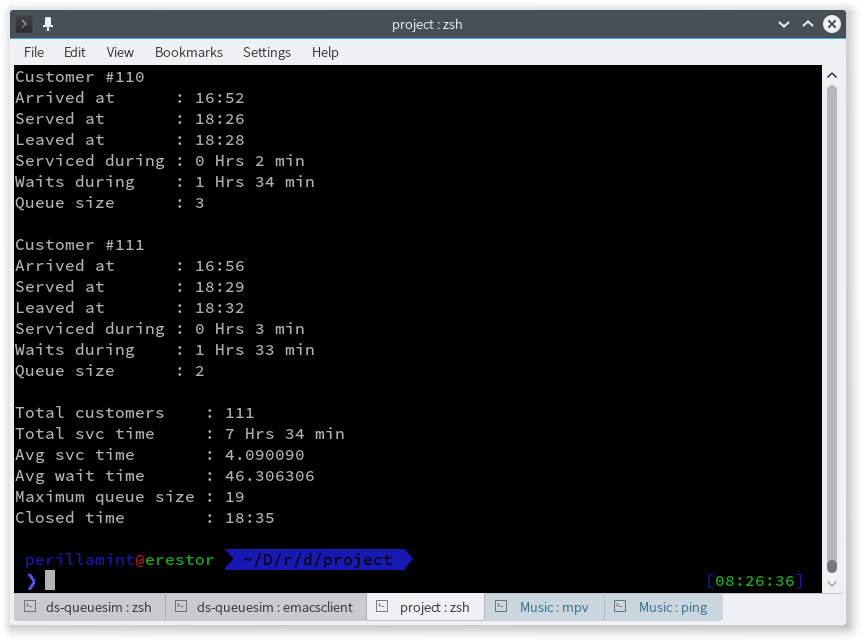
\includegraphics [width=120mm]{queuesim.png}
  \caption {}
  \label{fig:dmesg}
\end {figure}

\begin {figure}[h!]
  \centering
  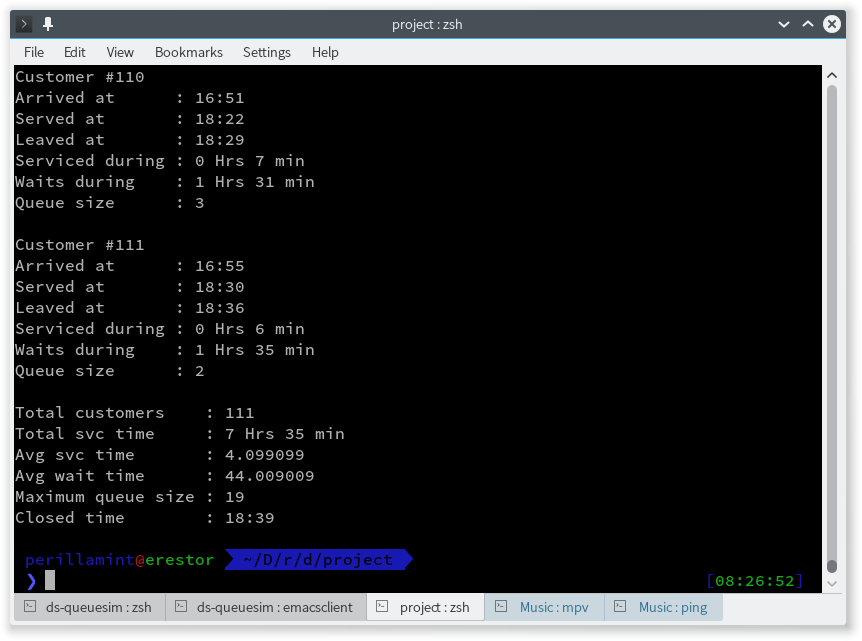
\includegraphics [width=120mm]{queuesim1.png}
  \caption {}
  \label{fig:dmesg}
\end {figure}

\begin {figure}[h!]
  \centering
  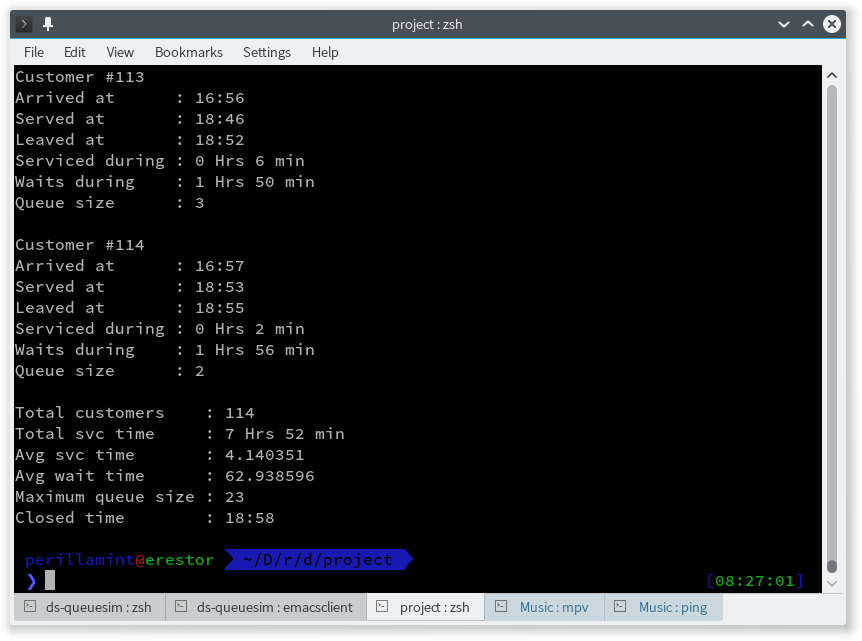
\includegraphics [width=120mm]{queuesim2.png}
  \caption {}
  \label{fig:dmesg}
\end {figure}

\newpage
\section {시뮬레이션 결과 - 조건 2}
조건 2: 3분당 1명꼴, 서버 두 명, 서비스 타임 1-7 분\newline
createDriver(60 * 9 + 0, 60 * 9 + 480, 3, 1, 7, 2);

\begin {figure}[h]
  \centering
  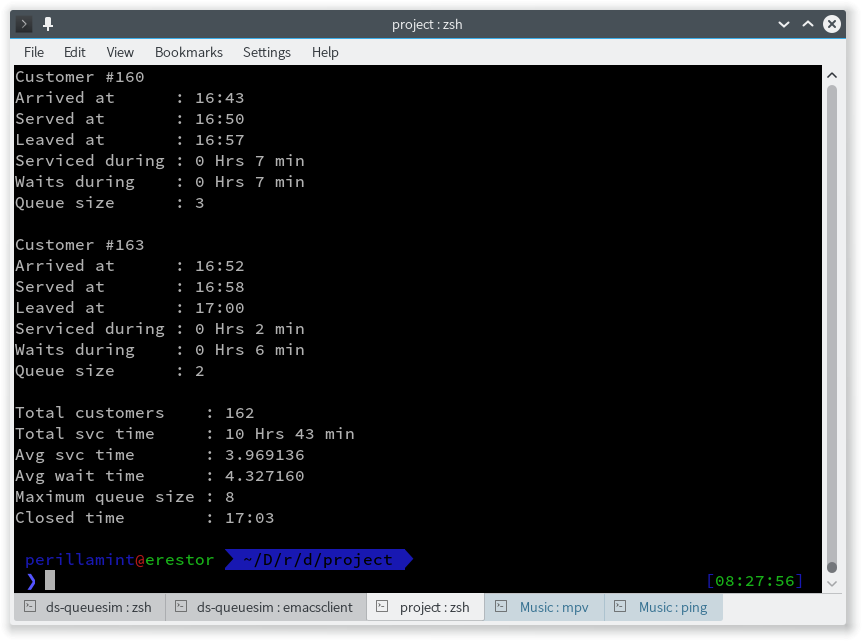
\includegraphics [width=120mm]{queuesim3.png}
  \caption {}
  \label{fig:dmesg}
\end {figure}

\begin {figure}[h]
  \centering
  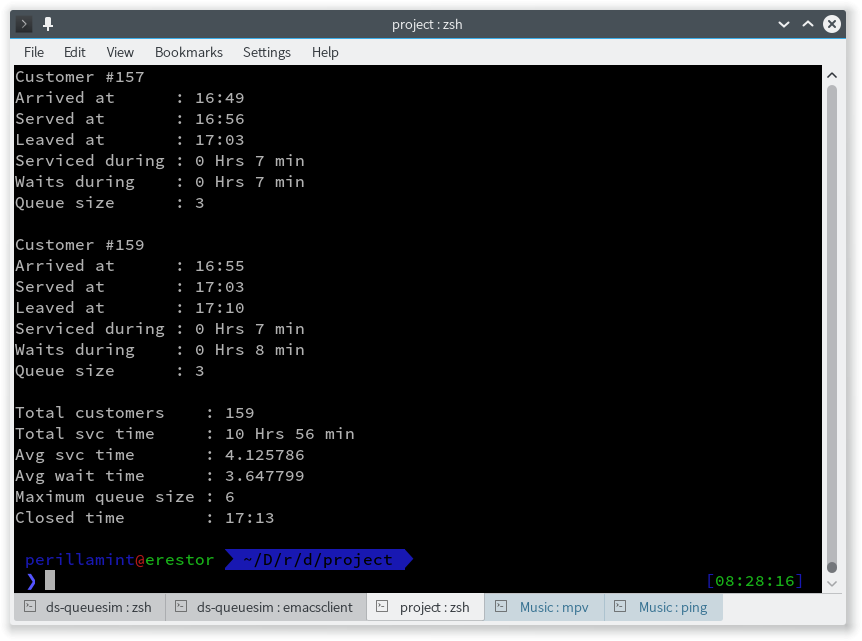
\includegraphics [width=120mm]{queuesim4.png}
  \caption {}
  \label{fig:dmesg}
\end {figure}

\begin {figure}[h]
  \centering
  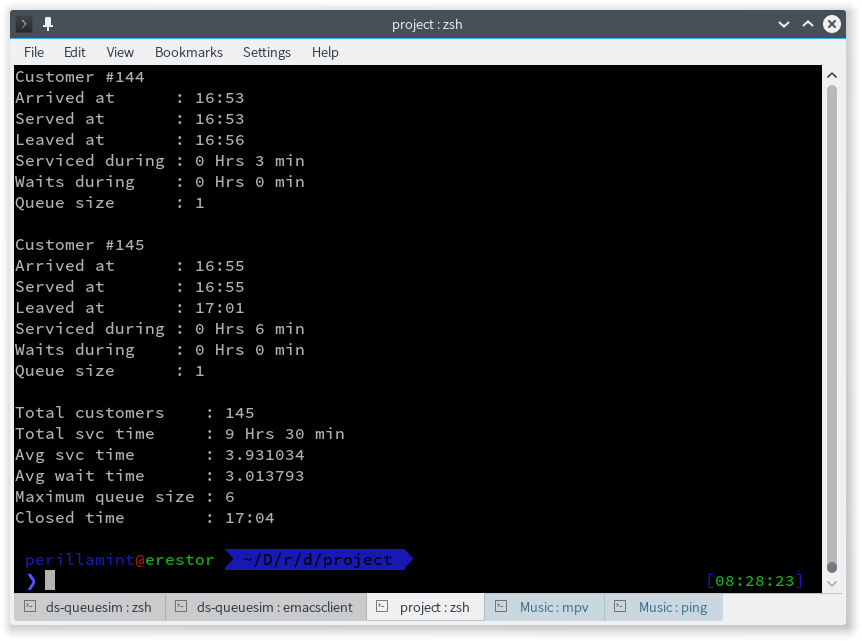
\includegraphics [width=120mm]{queuesim5.png}
  \caption {}
  \label{fig:dmesg}
\end {figure}

\end {document}
